\section{Loudspeaker}

In order to understand how the distortion occurs in a loudspeaker, it is necessary to understand the basic fundamentals and the topology of a loudspeaker. %This section will consist of the basic topology and then glans over the topic of vibration induced in the speaker woofer.

%\subsubsection*{The basics}
The loudspeaker is a transducer which purpose is to convert the electrical energy into acoustical energy. This is done by sending the signal into a loudspeaker which can consist of numerous drivers. The drivers are designed to perform best within their frequency range, hence they are usually different sizes in diameter.
\begin{itemize}
\item[] For the high frequencies, which is roughly 2 kHz and above, a tweeter is used of approximately 1 - 2 inches in diameter.
\item[] In the midrange, which is roughly 300 Hz to 200 - 2 kHz, a midrange driver is used of approximately 4 - 6 inches in diameter.
\item[] The lower frequencies, which is 200 Hz and below, is then handled by the woofer. The woofer is usually 5 - 6 inches and above in diameter.
\end{itemize}
The reason for different diameters in drivers is because of the wavelength of the specific frequencies. Should a woofer play frequencies at +4 kHz it would result in the driver physically not being able to move that fast. The limitations will end up in non-linear distortion in the diaphragm. Vice versa, should a tweeter reproduce low frequency sound at high \gls{SPL} it will end in distortion. %The tweeter has a very low excursion range which limits it to the high frequency area. 
Because the tweeter has a very low excursion range, which means it cannot break because of its physical movement only the woofer will be analyzed further. 

%\todo[inline]{Måske noget forklaring om det kun er nødvendigt at kigge på wooferen}


\subsection*{Diaphragm excursion}
When the speaker plays sound it does so by moving the diaphragm in the woofer. This difference in air pressure is then perceived as sound. The sound has a specific wavelength according to the frequency. This means that trying to move the air with a speaker cone is more efficient in a specific frequency area according to the diameter. %If a speaker with a small diameter tries to generate a large wavelength the sound would bend and escape around the edges. 
Since a large wavelength requires more air to be pushed, speaker cones is sized according to what area they are going to play.

Next, the woofer needs to deliver a sufficient \gls{SPL}. This creates the need for enough excursion of the diaphragm. Without dwelling to much on the speaker construction, the diaphragm is suspended in free air hold in place by the surround, see \autoref{fig:regularspeaker}, and the spider. The spider is a diaphragm holding the voice coil more tightly in place. 

\begin{figure}[H]
\centering
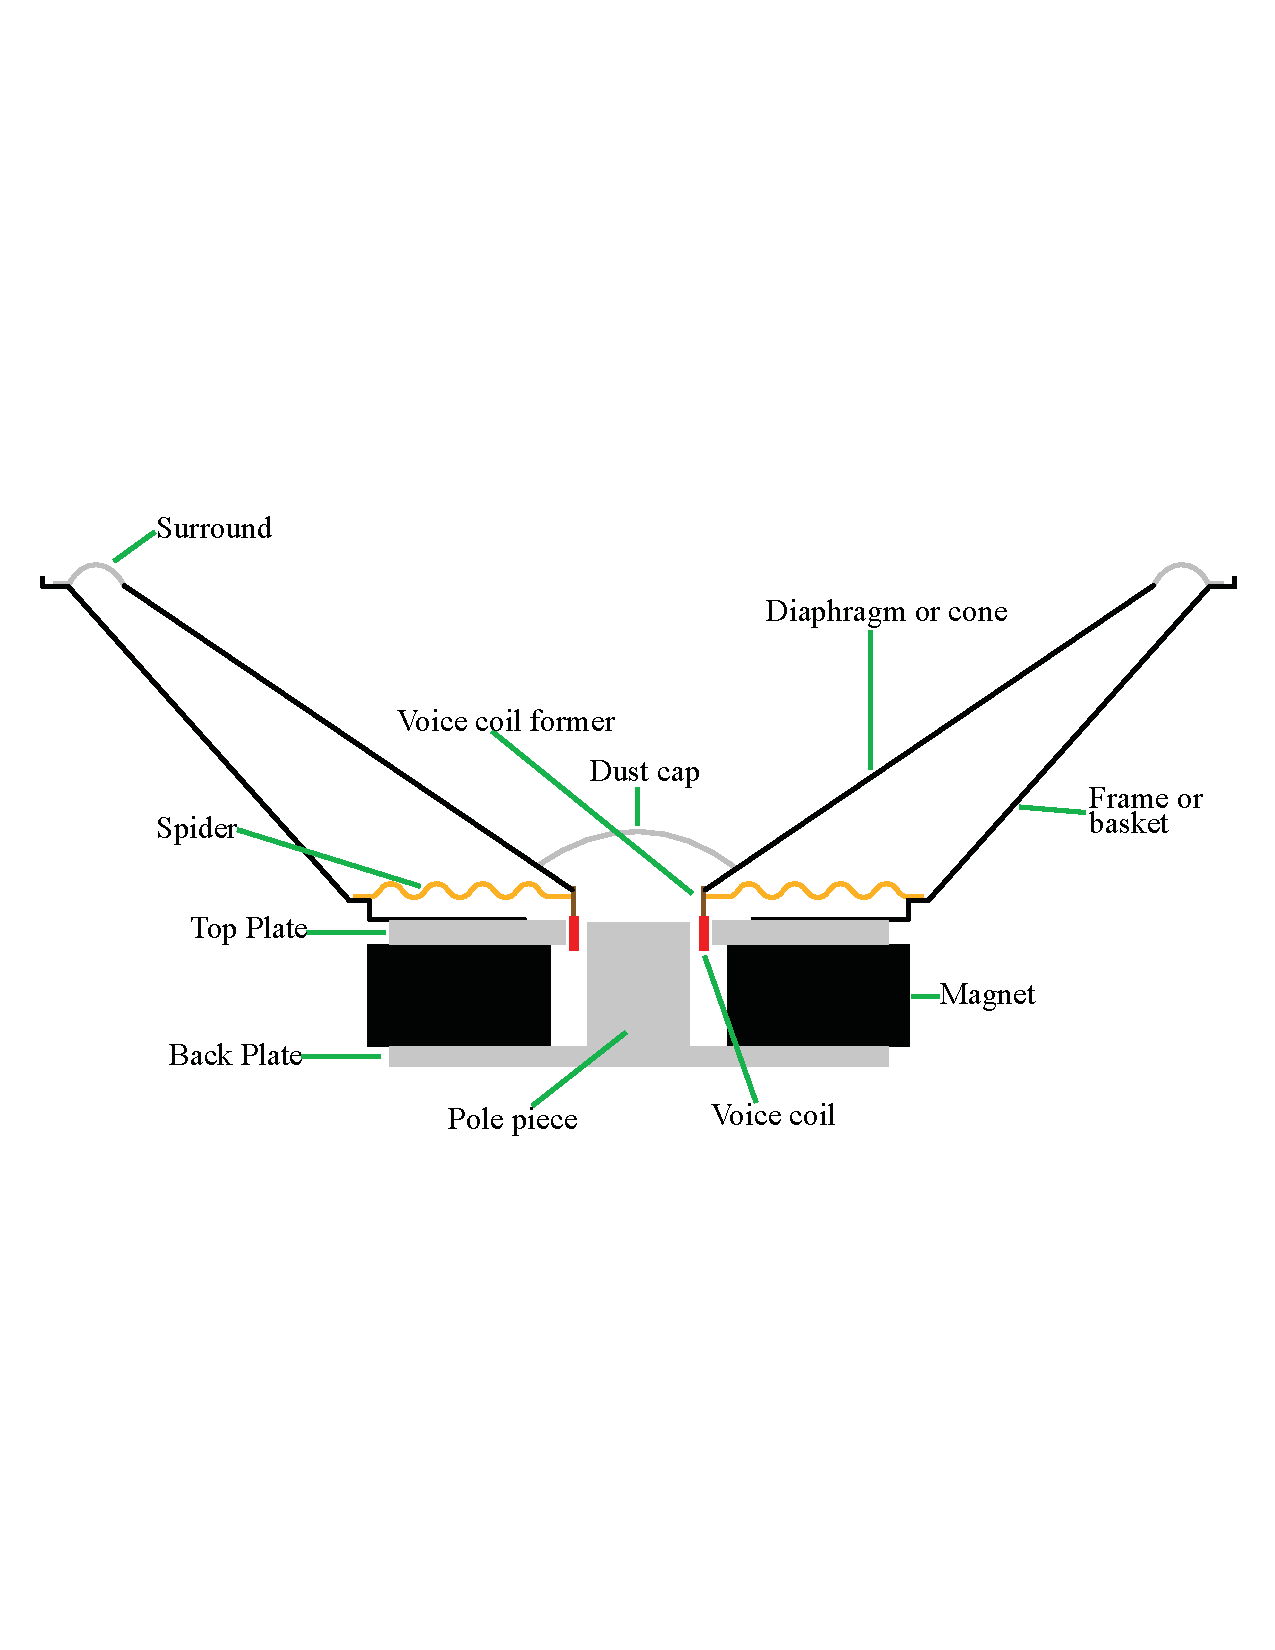
\includegraphics[width=0.75\textwidth]{Speaker-cross-section}
\caption{Cross section of a woofer.}
\label{fig:louderspeakerCrossSection}
\end{figure}

When the diaphragm moves it will have physical limits from the mechanical construction. At most, the diaphragm will move regular and linear. When the diaphragm is pushed to the boundaries, the limits of the mechanical construction will intervene and create non-linearities and distortion as seen in \autoref{fig:excursion_graph}. %This is discussed further in \autoref{subsec:impulses}.

\begin{figure}[H]
\centering
\tikzsetnextfilename{excursion_graph}
% This file was created by matlab2tikz.
%
%The latest updates can be retrieved from
%  http://www.mathworks.com/matlabcentral/fileexchange/22022-matlab2tikz-matlab2tikz
%where you can also make suggestions and rate matlab2tikz.
%
\begin{tikzpicture}

\begin{axis}[%
width=3.5in,
height=1.5in,
at={(1.011in,0.642in)},
scale only axis,
xmin=0,
xmax=10,
xticklabels={\empty},
xlabel={Current},
ymin=0,
ymax=9,
yticklabels={\empty},
ylabel={Excursion},
axis background/.style={fill=white},
legend style={legend cell align=left,align=left,draw=white!15!black}
]
\addplot [color=black,solid]
  table[row sep=crcr]{%
0	1.58644690201345e-05\\
0.01	0.0124029075014851\\
0.02	0.0248245010491709\\
0.03	0.0372795887296059\\
0.04	0.0497671348054388\\
0.05	0.0622861239177309\\
0.06	0.0748355608215229\\
0.07	0.087414470123661\\
0.08	0.100021896022872\\
0.09	0.112656902052075\\
0.1	0.125318570822912\\
0.11	0.138006003772496\\
0.12	0.150718320912349\\
0.13	0.163454660579537\\
0.14	0.176214179189965\\
0.15	0.188996050993848\\
0.16	0.20179946783332\\
0.17	0.214623638902183\\
0.18	0.227467790507789\\
0.19	0.24033116583502\\
0.2	0.253213024712385\\
0.21	0.266112643380189\\
0.22	0.279029314260798\\
0.23	0.291962345730951\\
0.24	0.304911061896135\\
0.25	0.317874802367002\\
0.26	0.330852922037808\\
0.27	0.343844790866878\\
0.28	0.356849793659072\\
0.29	0.369867329850245\\
0.3	0.382896813293693\\
0.31	0.395937672048568\\
0.32	0.408989348170249\\
0.33	0.42205129750267\\
0.34	0.435122989472575\\
0.35	0.448203906885702\\
0.36	0.461293545724884\\
0.37	0.474391414950042\\
0.38	0.487497036300082\\
0.39	0.500609944096661\\
0.4	0.513729685049826\\
0.41	0.526855818065511\\
0.42	0.539987914054878\\
0.43	0.553125555745492\\
0.44	0.566268337494321\\
0.45	0.57941586510255\\
0.46	0.592567755632195\\
0.47	0.605723637224506\\
0.48	0.618883148920154\\
0.49	0.632045940481182\\
0.5	0.645211672214722\\
0.51	0.658380014798443\\
0.52	0.671550649107758\\
0.53	0.684723266044735\\
0.54	0.697897566368738\\
0.55	0.711073260528765\\
0.56	0.724250068497479\\
0.57	0.737427719606927\\
0.58	0.750605952385929\\
0.59	0.763784514399125\\
0.6	0.77696316208768\\
0.61	0.790141660611627\\
0.62	0.803319783693839\\
0.63	0.816497313465622\\
0.64	0.829674040313922\\
0.65	0.842849762730126\\
0.66	0.856024287160453\\
0.67	0.869197427857931\\
0.68	0.882369006735931\\
0.69	0.895538853223273\\
0.7	0.908706804120867\\
0.71	0.921872703459909\\
0.72	0.935036402361586\\
0.73	0.94819775889832\\
0.74	0.961356637956503\\
0.75	0.974512911100743\\
0.76	0.987666456439594\\
0.77	1.00081715849276\\
0.78	1.01396490805979\\
0.79	1.02710960209018\\
0.8	1.04025114355502\\
0.81	1.05338944131995\\
0.82	1.06652441001967\\
0.83	1.07965596993382\\
0.84	1.09278404686423\\
0.85	1.10590857201363\\
0.86	1.11902948186577\\
0.87	1.13214671806683\\
0.88	1.14526022730829\\
0.89	1.15836996121112\\
0.9	1.17147587621137\\
0.91	1.18457793344702\\
0.92	1.19767609864625\\
0.93	1.21077034201702\\
0.94	1.22386063813791\\
0.95	1.23694696585034\\
0.96	1.25002930815207\\
0.97	1.26310765209194\\
0.98	1.27618198866595\\
0.99	1.28925231271461\\
1	1.30231862282149\\
1.01	1.31538092121313\\
1.02	1.32843921366005\\
1.03	1.34149350937918\\
1.04	1.3545438209373\\
1.05	1.36759016415593\\
1.06	1.38063255801721\\
1.07	1.39367102457117\\
1.08	1.40670558884402\\
1.09	1.41973627874781\\
1.1	1.43276312499105\\
1.11	1.44578616099069\\
1.12	1.45880542278518\\
1.13	1.47182094894859\\
1.14	1.48483278050605\\
1.15	1.49784096085019\\
1.16	1.51084553565872\\
1.17	1.52384655281318\\
1.18	1.53684406231872\\
1.19	1.54983811622509\\
1.2	1.56282876854857\\
1.21	1.5758160751951\\
1.22	1.58880009388446\\
1.23	1.60178088407545\\
1.24	1.61475850689225\\
1.25	1.62773302505168\\
1.26	1.64070450279161\\
1.27	1.65367300580038\\
1.28	1.66663860114723\\
1.29	1.67960135721372\\
1.3	1.69256134362623\\
1.31	1.70551863118938\\
1.32	1.71847329182052\\
1.33	1.73142539848513\\
1.34	1.74437502513328\\
1.35	1.75732224663695\\
1.36	1.77026713872846\\
1.37	1.78320977793967\\
1.38	1.79615024154231\\
1.39	1.80908860748912\\
1.4	1.82202495435596\\
1.41	1.83495936128487\\
1.42	1.84789190792802\\
1.43	1.86082267439254\\
1.44	1.87375174118634\\
1.45	1.8866791891647\\
1.46	1.89960509947785\\
1.47	1.91252955351938\\
1.48	1.92545263287553\\
1.49	1.93837441927533\\
1.5	1.95129499454163\\
1.51	1.96421444054295\\
1.52	1.97713283914617\\
1.53	1.99005027217008\\
1.54	2.00296682133972\\
1.55	2.0158825682416\\
1.56	2.02879759427965\\
1.57	2.04171198063206\\
1.58	2.05462580820885\\
1.59	2.06753915761027\\
1.6	2.080452109086\\
1.61	2.09336474249508\\
1.62	2.10627713726664\\
1.63	2.1191893723614\\
1.64	2.13210152623389\\
1.65	2.14501367679549\\
1.66	2.15792590137816\\
1.67	2.17083827669888\\
1.68	2.18375087882492\\
1.69	2.19666378313973\\
1.7	2.20957706430959\\
1.71	2.222490796251\\
1.72	2.23540505209873\\
1.73	2.24831990417456\\
1.74	2.26123542395675\\
1.75	2.27415168205019\\
1.76	2.28706874815719\\
1.77	2.29998669104895\\
1.78	2.31290557853775\\
1.79	2.32582547744974\\
1.8	2.33874645359839\\
1.81	2.35166857175858\\
1.82	2.36459189564139\\
1.83	2.37751648786945\\
1.84	2.39044240995292\\
1.85	2.40336972226617\\
1.86	2.41629848402498\\
1.87	2.42922875326437\\
1.88	2.44216058681712\\
1.89	2.45509404029273\\
1.9	2.46802916805713\\
1.91	2.48096602321284\\
1.92	2.49390465757982\\
1.93	2.50684512167679\\
1.94	2.51978746470323\\
1.95	2.53273173452179\\
1.96	2.54567797764143\\
1.97	2.55862623920097\\
1.98	2.57157656295322\\
1.99	2.58452899124972\\
2	2.59748356502587\\
2.01	2.61044032378676\\
2.02	2.62339930559334\\
2.03	2.63636054704922\\
2.04	2.64932408328799\\
2.05	2.66228994796094\\
2.06	2.67525817322538\\
2.07	2.68822878973339\\
2.08	2.70120182662109\\
2.09	2.71417731149837\\
2.1	2.72715527043912\\
2.11	2.74013572797189\\
2.12	2.75311870707106\\
2.13	2.76610422914844\\
2.14	2.7790923140453\\
2.15	2.79208298002496\\
2.16	2.80507624376564\\
2.17	2.81807212035396\\
2.18	2.83107062327865\\
2.19	2.84407176442491\\
2.2	2.857075554069\\
2.21	2.8700820008734\\
2.22	2.88309111188223\\
2.23	2.89610289251726\\
2.24	2.90911734657415\\
2.25	2.92213447621918\\
2.26	2.93515428198636\\
2.27	2.94817676277491\\
2.28	2.96120191584714\\
2.29	2.97422973682669\\
2.3	2.98726021969714\\
2.31	3.00029335680102\\
2.32	3.01332913883917\\
2.33	3.02636755487039\\
2.34	3.03940859231157\\
2.35	3.05245223693805\\
2.36	3.06549847288441\\
2.37	3.07854728264554\\
2.38	3.09159864707806\\
2.39	3.10465254540209\\
2.4	3.11770895520333\\
2.41	3.13076785243547\\
2.42	3.14382921142287\\
2.43	3.15689300486364\\
2.44	3.16995920383292\\
2.45	3.18302777778657\\
2.46	3.19609869456505\\
2.47	3.20917192039772\\
2.48	3.22224741990729\\
2.49	3.23532515611464\\
2.5	3.24840509044392\\
2.51	3.26148718272792\\
2.52	3.27457139121365\\
2.53	3.28765767256827\\
2.54	3.30074598188528\\
2.55	3.31383627269086\\
2.56	3.32692849695063\\
2.57	3.34002260507653\\
2.58	3.353118545934\\
2.59	3.36621626684937\\
2.6	3.37931571361758\\
2.61	3.39241683051\\
2.62	3.40551956028258\\
2.63	3.41862384418419\\
2.64	3.43172962196516\\
2.65	3.44483683188612\\
2.66	3.45794541072695\\
2.67	3.471055293796\\
2.68	3.48416641493952\\
2.69	3.49727870655127\\
2.7	3.51039209958235\\
2.71	3.52350652355117\\
2.72	3.53662190655372\\
2.73	3.54973817527392\\
2.74	3.5628552549942\\
2.75	3.57597306960627\\
2.76	3.58909154162203\\
2.77	3.60221059218473\\
2.78	3.61533014108016\\
2.79	3.62845010674818\\
2.8	3.64157040629427\\
2.81	3.6546909555013\\
2.82	3.66781166884147\\
2.83	3.68093245948834\\
2.84	3.6940532393291\\
2.85	3.70717391897688\\
2.86	3.72029440778328\\
2.87	3.73341461385104\\
2.88	3.74653444404673\\
2.89	3.75965380401376\\
2.9	3.77277259818535\\
2.91	3.7858907297977\\
2.92	3.79900810090329\\
2.93	3.81212461238427\\
2.94	3.82524016396596\\
2.95	3.8383546542305\\
2.96	3.85146798063056\\
2.97	3.86458003950321\\
2.98	3.87769072608383\\
2.99	3.89079993452016\\
3	3.90390755788646\\
3.01	3.91701348819771\\
3.02	3.93011761642394\\
3.03	3.94321983250465\\
3.04	3.95632002536328\\
3.05	3.9694180829218\\
3.06	3.98251389211533\\
3.07	3.9956073389069\\
3.08	4.00869830830224\\
3.09	4.02178668436463\\
3.1	4.03487235022984\\
3.11	4.04795518812113\\
3.12	4.06103507936431\\
3.13	4.07411190440285\\
3.14	4.08718554281304\\
3.15	4.10025587331924\\
3.16	4.11332277380914\\
3.17	4.12638612134906\\
3.18	4.13944579219937\\
3.19	4.15250166182982\\
3.2	4.16555360493507\\
3.21	4.17860149545009\\
3.22	4.19164520656574\\
3.23	4.2046846107443\\
3.24	4.21771957973505\\
3.25	4.23074998458984\\
3.26	4.24377569567877\\
3.27	4.25679658270582\\
3.28	4.2698125147245\\
3.29	4.28282336015357\\
3.3	4.2958289867927\\
3.31	4.30882926183823\\
3.32	4.32182405189884\\
3.33	4.33481322301133\\
3.34	4.34779664065631\\
3.35	4.36077416977396\\
3.36	4.37374567477976\\
3.37	4.38671101958024\\
3.38	4.39967006758868\\
3.39	4.41262268174086\\
3.4	4.42556872451078\\
3.41	4.43850805792634\\
3.42	4.45144054358506\\
3.43	4.46436604266974\\
3.44	4.47728441596413\\
3.45	4.49019552386856\\
3.46	4.50309922641559\\
3.47	4.51599538328558\\
3.48	4.52888385382226\\
3.49	4.54176449704832\\
3.5	4.55463717168086\\
3.51	4.56750173614692\\
3.52	4.58035804859894\\
3.53	4.59320596693014\\
3.54	4.60604534878993\\
3.55	4.61887605159926\\
3.56	4.63169793256587\\
3.57	4.64451084869963\\
3.58	4.65731465682768\\
3.59	4.67010921360964\\
3.6	4.68289437555274\\
3.61	4.69566999902685\\
3.62	4.70843594027955\\
3.63	4.72119205545108\\
3.64	4.73393820058922\\
3.65	4.74667423166423\\
3.66	4.75940000458355\\
3.67	4.77211537520663\\
3.68	4.78482019935955\\
3.69	4.79751433284966\\
3.7	4.81019763148015\\
3.71	4.82286995106449\\
3.72	4.8355311474409\\
3.73	4.84818107648668\\
3.74	4.86081959413249\\
3.75	4.87344655637654\\
3.76	4.88606181929878\\
3.77	4.89866523907491\\
3.78	4.91125667199037\\
3.79	4.9238359744543\\
3.8	4.9364030030133\\
3.81	4.94895761436522\\
3.82	4.96149966537282\\
3.83	4.97402901307734\\
3.84	4.98654551471204\\
3.85	4.99904902771556\\
3.86	5.0115394097453\\
3.87	5.02401651869061\\
3.88	5.03648021268601\\
3.89	5.04893035012419\\
3.9	5.06136678966898\\
3.91	5.07378939026829\\
3.92	5.08619801116683\\
3.93	5.09859251191882\\
3.94	5.11097275240058\\
3.95	5.12333859282305\\
3.96	5.13568989374415\\
3.97	5.14802651608108\\
3.98	5.16034832112255\\
3.99	5.17265517054086\\
4	5.18494692640388\\
4.01	5.19722345118694\\
4.02	5.20948460778466\\
4.03	5.22173025952257\\
4.04	5.23396027016871\\
4.05	5.24617450394513\\
4.06	5.25837282553918\\
4.07	5.27055510011482\\
4.08	5.28272119332376\\
4.09	5.29487097131642\\
4.1	5.30700430075294\\
4.11	5.31912104881395\\
4.12	5.33122108321122\\
4.13	5.3433042721983\\
4.14	5.35537048458097\\
4.15	5.36741958972757\\
4.16	5.37945145757926\\
4.17	5.39146595866011\\
4.18	5.4034629640871\\
4.19	5.41544234558004\\
4.2	5.42740397547129\\
4.21	5.43934772671541\\
4.22	5.45127347289871\\
4.23	5.46318108824861\\
4.24	5.47507044764295\\
4.25	5.48694142661914\\
4.26	5.4987939013832\\
4.27	5.51062774881866\\
4.28	5.52244284649537\\
4.29	5.53423907267815\\
4.3	5.54601630633534\\
4.31	5.5577744271472\\
4.32	5.56951331551423\\
4.33	5.58123285256529\\
4.34	5.59293292016569\\
4.35	5.60461340092507\\
4.36	5.61627417820517\\
4.37	5.62791513612754\\
4.38	5.63953615958101\\
4.39	5.65113713422912\\
4.4	5.66271794651739\\
4.41	5.67427848368046\\
4.42	5.6858186337491\\
4.43	5.69733828555709\\
4.44	5.70883732874799\\
4.45	5.72031565378175\\
4.46	5.7317731519412\\
4.47	5.74320971533842\\
4.48	5.75462523692099\\
4.49	5.76601961047803\\
4.5	5.77739273064626\\
4.51	5.78874449291575\\
4.52	5.80007479363568\\
4.53	5.81138353001989\\
4.54	5.82267060015235\\
4.55	5.83393590299243\\
4.56	5.84517933838012\\
4.57	5.85640080704105\\
4.58	5.86760021059141\\
4.59	5.87877745154273\\
4.6	5.88993243330655\\
4.61	5.90106506019889\\
4.62	5.91217523744471\\
4.63	5.92326287118208\\
4.64	5.93432786846633\\
4.65	5.9453701372741\\
4.66	5.95638958650708\\
4.67	5.96738612599582\\
4.68	5.9783596665033\\
4.69	5.98931011972837\\
4.7	6.00023739830909\\
4.71	6.01114141582594\\
4.72	6.02202208680484\\
4.73	6.03287932672014\\
4.74	6.04371305199736\\
4.75	6.05452318001589\\
4.76	6.06530962911152\\
4.77	6.07607231857889\\
4.78	6.08681116867367\\
4.79	6.09752610061478\\
4.8	6.1082170365864\\
4.81	6.1188838997398\\
4.82	6.12952661419517\\
4.83	6.14014510504319\\
4.84	6.15073929834654\\
4.85	6.16130912114127\\
4.86	6.17185450143803\\
4.87	6.18237536822322\\
4.88	6.19287165145988\\
4.89	6.20334328208865\\
4.9	6.21379019202841\\
4.91	6.22421231417695\\
4.92	6.23460958241139\\
4.93	6.24498193158853\\
4.94	6.25532929754511\\
4.95	6.26565161709787\\
4.96	6.27594882804351\\
4.97	6.28622086915859\\
4.98	6.29646768019922\\
4.99	6.30668920190059\\
5	6.31688537597656\\
5.01	6.32705614511898\\
5.02	6.33720145299685\\
5.03	6.34732124425551\\
5.04	6.35741546451558\\
5.05	6.36748406037185\\
5.06	6.37752697939201\\
5.07	6.3875441701153\\
5.08	6.39753558205098\\
5.09	6.40750116567676\\
5.1	6.41744087243705\\
5.11	6.42735465474111\\
5.12	6.4372424659611\\
5.13	6.44710426043001\\
5.14	6.45693999343944\\
5.15	6.46674962123731\\
5.16	6.47653310102546\\
5.17	6.48629039095704\\
5.18	6.49602145013397\\
5.19	6.5057262386041\\
5.2	6.51540471735836\\
5.21	6.52505684832778\\
5.22	6.53468259438041\\
5.23	6.54428191931811\\
5.24	6.55385478787324\\
5.25	6.56340116570525\\
5.26	6.57292101939716\\
5.27	6.5824143164519\\
5.28	6.59188102528864\\
5.29	6.60132111523889\\
5.3	6.61073455654258\\
5.31	6.62012132034403\\
5.32	6.62948137868777\\
5.33	6.63881470451434\\
5.34	6.6481212716559\\
5.35	6.65740105483178\\
5.36	6.66665402964398\\
5.37	6.67588017257248\\
5.38	6.68507946097051\\
5.39	6.69425187305972\\
5.4	6.70339738792526\\
5.41	6.71251598551073\\
5.42	6.72160764661308\\
5.43	6.73067235287738\\
5.44	6.73971008679156\\
5.45	6.74872083168092\\
5.46	6.75770457170278\\
5.47	6.76666129184078\\
5.48	6.77559097789937\\
5.49	6.78449361649789\\
5.5	6.79336919506489\\
5.51	6.80221770183211\\
5.52	6.81103912582857\\
5.53	6.81983345687438\\
5.54	6.82860068557475\\
5.55	6.83734080331352\\
5.56	6.84605380224705\\
5.57	6.85473967529766\\
5.58	6.86339841614731\\
5.59	6.87203001923086\\
5.6	6.88063447972962\\
5.61	6.88921179356453\\
5.62	6.8977619573894\\
5.63	6.90628496858416\\
5.64	6.9147808252478\\
5.65	6.92324952619146\\
5.66	6.93169107093145\\
5.67	6.94010545968189\\
5.68	6.94849269334782\\
5.69	6.95685277351774\\
5.7	6.96518570245633\\
5.71	6.97349148309714\\
5.72	6.98177011903507\\
5.73	6.99002161451894\\
5.74	6.99824597444381\\
5.75	7.00644320434355\\
5.76	7.01461331038295\\
5.77	7.02275629935019\\
5.78	7.03087217864884\\
5.79	7.03896095629029\\
5.8	7.0470226408856\\
5.81	7.05505724163768\\
5.82	7.06306476833336\\
5.83	7.07104523133521\\
5.84	7.07899864157359\\
5.85	7.08692501053836\\
5.86	7.09482435027093\\
5.87	7.10269667335588\\
5.88	7.11054199291264\\
5.89	7.11836032258746\\
5.9	7.12615167654478\\
5.91	7.13391606945899\\
5.92	7.14165351650605\\
5.93	7.149364033355\\
5.94	7.15704763615943\\
5.95	7.16470434154903\\
5.96	7.17233416662104\\
5.97	7.17993712893172\\
5.98	7.18751324648755\\
5.99	7.1950625377369\\
6	7.20258502156111\\
6.01	7.21008071726598\\
6.02	7.21754964457304\\
6.03	7.22499182361064\\
6.04	7.23240727490554\\
6.05	7.23979601937387\\
6.06	7.24715807831246\\
6.07	7.25449347339005\\
6.08	7.26180222663848\\
6.09	7.26908436044379\\
6.1	7.27633989753748\\
6.11	7.28356886098764\\
6.12	7.29077127419005\\
6.13	7.29794716085942\\
6.14	7.30509654502037\\
6.15	7.31221945099868\\
6.16	7.31931590341239\\
6.17	7.32638592716295\\
6.18	7.33342954742625\\
6.19	7.34044678964373\\
6.2	7.34743767951376\\
6.21	7.35440224298253\\
6.22	7.36134050623509\\
6.23	7.36825249568695\\
6.24	7.3751382379746\\
6.25	7.38199775994732\\
6.26	7.38883108865786\\
6.27	7.3956382513539\\
6.28	7.40241927546912\\
6.29	7.40917418861458\\
6.3	7.41590301856969\\
6.31	7.42260579327378\\
6.32	7.42928254081715\\
6.33	7.43593328943242\\
6.34	7.44255806748601\\
6.35	7.44915690346927\\
6.36	7.45572982598997\\
6.37	7.46227686376367\\
6.38	7.46879804560521\\
6.39	7.47529340042012\\
6.4	7.48176295719618\\
6.41	7.48820674499488\\
6.42	7.494624792943\\
6.43	7.50101713022435\\
6.44	7.50738378607132\\
6.45	7.51372478975639\\
6.46	7.52004017058429\\
6.47	7.52632995788335\\
6.48	7.5325941809976\\
6.49	7.53883286927852\\
6.5	7.54504605207703\\
6.51	7.55123375873532\\
6.52	7.55739601857898\\
6.53	7.56353286090925\\
6.54	7.56964431499469\\
6.55	7.57573041006389\\
6.56	7.58179117529728\\
6.57	7.58782663981972\\
6.58	7.59383683269278\\
6.59	7.5998217829072\\
6.6	7.60578151937525\\
6.61	7.61171607092349\\
6.62	7.61762546628531\\
6.63	7.62350973409354\\
6.64	7.62936890287349\\
6.65	7.63520300103547\\
6.66	7.64101205686793\\
6.67	7.6467960985304\\
6.68	7.65255515404654\\
6.69	7.65828925129728\\
6.7	7.66399841801426\\
6.71	7.66968268177274\\
6.72	7.67534206998537\\
6.73	7.68097660989559\\
6.74	7.68658632857112\\
6.75	7.69217125289767\\
6.76	7.69773140957278\\
6.77	7.70326682509957\\
6.78	7.70877752578066\\
6.79	7.71426353771233\\
6.8	7.71972488677858\\
6.81	7.72516159864544\\
6.82	7.73057369875516\\
6.83	7.73596121232083\\
6.84	7.74132416432083\\
6.85	7.74666257949352\\
6.86	7.75197648233196\\
6.87	7.75726589707882\\
6.88	7.7625308477213\\
6.89	7.76777135798636\\
6.9	7.77298745133577\\
6.91	7.77817915096152\\
6.92	7.78334647978125\\
6.93	7.78848946043371\\
6.94	7.79360811527472\\
6.95	7.79870246637274\\
6.96	7.80377253550464\\
6.97	7.80881834415228\\
6.98	7.81383991349816\\
6.99	7.81883726442204\\
7	7.82381041749725\\
7.01	7.82875939298735\\
7.02	7.8336842108427\\
7.03	7.83858489069758\\
7.04	7.8434614518668\\
7.05	7.84831391334314\\
7.06	7.85314229379447\\
7.07	7.85794661156106\\
7.08	7.86272688465343\\
7.09	7.86748313074977\\
7.1	7.87221536719389\\
7.11	7.87692361099304\\
7.12	7.8816078788165\\
7.13	7.8862681869934\\
7.14	7.89090455151134\\
7.15	7.89551698801509\\
7.16	7.90010551180519\\
7.17	7.90467013783701\\
7.18	7.90921088071987\\
7.19	7.91372775471599\\
7.2	7.91822077374029\\
7.21	7.92268995135961\\
7.22	7.92713530079272\\
7.23	7.93155683491024\\
7.24	7.93595456623439\\
7.25	7.94032850693964\\
7.26	7.94467866885286\\
7.27	7.94900506345412\\
7.28	7.95330770187735\\
7.29	7.95758659491131\\
7.3	7.96184175300086\\
7.31	7.96607318624804\\
7.32	7.97028090441384\\
7.33	7.97446491691973\\
7.34	7.97862523284942\\
7.35	7.98276186095143\\
7.36	7.98687480964076\\
7.37	7.99096408700157\\
7.38	7.99502970078997\\
7.39	7.99907165843674\\
7.4	8.00308996705014\\
7.41	8.00708463341969\\
7.42	8.01105566401894\\
7.43	8.0150030650097\\
7.44	8.01892684224554\\
7.45	8.02282700127591\\
7.46	8.02670354735024\\
7.47	8.03055648542293\\
7.48	8.03438582015727\\
7.49	8.03819155593083\\
7.5	8.04197369684052\\
7.51	8.04573224670763\\
7.52	8.04946720908364\\
7.53	8.0531785872557\\
7.54	8.05686638425281\\
7.55	8.06053060285203\\
7.56	8.06417124558437\\
7.57	8.06778831474244\\
7.58	8.07138181238596\\
7.59	8.07495174035014\\
7.6	8.07849810025209\\
7.61	8.08202089349876\\
7.62	8.08552012129462\\
7.63	8.08899578464953\\
7.64	8.09244788438729\\
7.65	8.0958764211539\\
7.66	8.09928139542613\\
7.67	8.10266280752091\\
7.68	8.10602065760381\\
7.69	8.10935494569942\\
7.7	8.11266567170026\\
7.71	8.11595283537697\\
7.72	8.11921643638845\\
7.73	8.12245647429228\\
7.74	8.12567294855569\\
7.75	8.12886585856564\\
7.76	8.13203520364117\\
7.77	8.13518098304381\\
7.78	8.13830319598969\\
7.79	8.1414018416615\\
7.8	8.14447691922073\\
7.81	8.14752842781983\\
7.82	8.15055636661539\\
7.83	8.15356073478058\\
7.84	8.1565415315189\\
7.85	8.15949875607747\\
7.86	8.16243240776064\\
7.87	8.16534248594436\\
7.88	8.1682289900904\\
7.89	8.17109191976076\\
7.9	8.17393127463289\\
7.91	8.17674705451444\\
7.92	8.17953925935895\\
7.93	8.18230788928152\\
7.94	8.18505294457446\\
7.95	8.18777442572413\\
7.96	8.19047233342711\\
7.97	8.19314666860672\\
7.98	8.19579743243086\\
7.99	8.19842462632886\\
8	8.20102825200929\\
8.01	8.20360831147791\\
8.02	8.2061648070561\\
8.03	8.20869774139899\\
8.04	8.21120711751479\\
8.05	8.21369293878374\\
8.06	8.21615520897722\\
8.07	8.21859393227795\\
8.08	8.22100911330004\\
8.09	8.22340075710846\\
8.1	8.22576886924098\\
8.11	8.22811345572797\\
8.12	8.2304345231142\\
8.13	8.23273207848032\\
8.14	8.2350061294646\\
8.15	8.23725668428472\\
8.16	8.23948375176128\\
8.17	8.24168734133913\\
8.18	8.24386746311187\\
8.19	8.2460241278439\\
8.2	8.24815734699543\\
8.21	8.25026713274533\\
8.22	8.25235349801613\\
8.23	8.25441645649857\\
8.24	8.25645602267654\\
8.25	8.258472211852\\
8.26	8.26046504017148\\
8.27	8.26243452465071\\
8.28	8.264380683202\\
8.29	8.26630353466044\\
8.3	8.26820309881071\\
8.31	8.27007939641413\\
8.32	8.27193244923675\\
8.33	8.27376228007663\\
8.34	8.27556891279239\\
8.35	8.27735237233194\\
8.36	8.27911268476088\\
8.37	8.2808498772919\\
8.38	8.28256397831436\\
8.39	8.28425501742429\\
8.4	8.28592302545426\\
8.41	8.28756803450436\\
8.42	8.28919007797283\\
8.43	8.29078919058701\\
8.44	8.29236540843561\\
8.45	8.29391876900003\\
8.46	8.29544931118682\\
8.47	8.2969570753603\\
8.48	8.29844210337554\\
8.49	8.29990443861131\\
8.5	8.30134412600427\\
8.51	8.30276121208261\\
8.52	8.30415574500013\\
8.53	8.30552777457175\\
8.54	8.30687735230734\\
8.55	8.30820453144845\\
8.56	8.30950936700276\\
8.57	8.31079191578141\\
8.58	8.31205223643402\\
8.59	8.31329038948684\\
8.6	8.31450643737944\\
8.61	8.31570044450156\\
8.62	8.3168724772319\\
8.63	8.31802260397572\\
8.64	8.31915089520428\\
8.65	8.32025742349256\\
8.66	8.32134226355948\\
8.67	8.32240549230728\\
8.68	8.32344718886144\\
8.69	8.32446743461136\\
8.7	8.32546631325101\\
8.71	8.32644391082005\\
8.72	8.32740031574482\\
8.73	8.32833561888136\\
8.74	8.3292499135568\\
8.75	8.33014329561163\\
8.76	8.33101586344385\\
8.77	8.33186771805083\\
8.78	8.33269896307475\\
8.79	8.33350970484502\\
8.8	8.33430005242354\\
8.81	8.33507011765001\\
8.82	8.33582001518579\\
8.83	8.33654986256065\\
8.84	8.33725978021808\\
8.85	8.33794989156256\\
8.86	8.33862032300444\\
8.87	8.33927120400874\\
8.88	8.33990266714227\\
8.89	8.34051484812064\\
8.9	8.34110788585724\\
8.91	8.34168192251134\\
8.92	8.34223710353791\\
8.93	8.34277357773587\\
8.94	8.34329149729876\\
8.95	8.343791017864\\
8.96	8.3442722985639\\
8.97	8.34473550207676\\
8.98	8.34518079467768\\
8.99	8.3456083462902\\
9	8.34601833053889\\
9.01	8.34641092480066\\
9.02	8.34678631025891\\
9.03	8.34714467195592\\
9.04	8.34748619884608\\
9.05	8.3478110838513\\
9.06	8.34811952391333\\
9.07	8.34841172005023\\
9.08	8.34868787741044\\
9.09	8.34894820532894\\
9.1	8.34919291738269\\
9.11	8.34942223144661\\
9.12	8.34963636975158\\
9.13	8.34983555894004\\
9.14	8.35002003012416\\
9.15	8.35019001894363\\
9.16	8.35034576562369\\
9.17	8.35048751503385\\
9.18	8.35061551674676\\
9.19	8.35073002509828\\
9.2	8.35083129924593\\
9.21	8.35091960323084\\
9.22	8.35099520603639\\
9.23	8.35105838165118\\
9.24	8.35110940912861\\
9.25	8.35114857264911\\
9.26	8.35117616158371\\
9.27	8.35119247055479\\
9.28	8.35119779949884\\
9.29	8.35119245373186\\
9.3	8.35117674401145\\
9.31	8.35115098660051\\
9.32	8.35111550333329\\
9.33	8.35107062167906\\
9.34	8.35101667480782\\
9.35	8.35095400165596\\
9.36	8.35088294699273\\
9.37	8.35080386148535\\
9.38	8.35071710176765\\
9.39	8.35062303050595\\
9.4	8.35052201646786\\
9.41	8.3504144345885\\
9.42	8.35030066604141\\
9.43	8.35018109830472\\
9.44	8.35005612523292\\
9.45	8.3499261471248\\
9.46	8.34979157079287\\
9.47	8.34965280963622\\
9.48	8.34951028370913\\
9.49	8.34936441979264\\
9.5	8.34921565146701\\
9.51	8.34906441918269\\
9.52	8.34891117033257\\
9.53	8.34875635932651\\
9.54	8.34860044766135\\
9.55	8.34844390399815\\
9.56	8.34828720423223\\
9.57	8.34813083157098\\
9.58	8.34797527660525\\
9.59	8.34782103738786\\
9.6	8.34766861950646\\
9.61	8.34751853616006\\
9.62	8.34737130823622\\
9.63	8.34722746438551\\
9.64	8.34708754110184\\
9.65	8.34695208279602\\
9.66	8.34682164187649\\
9.67	8.34669677882662\\
9.68	8.34657806228264\\
9.69	8.34646606911291\\
9.7	8.34636138449792\\
9.71	8.34626460200964\\
9.72	8.34617632369042\\
9.73	8.34609716013545\\
9.74	8.34602773057233\\
9.75	8.3459686629427\\
9.76	8.345920593984\\
9.77	8.34588416931102\\
9.78	8.34586004349815\\
9.79	8.34584888016384\\
9.8	8.34585135205125\\
9.81	8.34586814111308\\
9.82	8.34589993859683\\
9.83	8.34594744512553\\
9.84	8.34601137078555\\
9.85	8.34609243521044\\
9.86	8.34619136766703\\
9.87	8.34630890713896\\
9.88	8.34644580241632\\
9.89	8.34660281217912\\
9.9	8.34678070508654\\
9.91	8.3469802598619\\
9.92	8.34720226538129\\
9.93	8.34744752076343\\
9.94	8.34771683545445\\
9.95	8.34801102931912\\
9.96	8.34833093273019\\
9.97	8.34867738665531\\
9.98	8.34905124275007\\
9.99	8.3494533634458\\
10	8.34988462204114\\
};
%\addlegendentry{fitted curve};
\end{axis}
\end{tikzpicture}%
\caption{General linearity curve of a loudspeaker.}
\label{fig:excursion_graph}
\end{figure}





\subsection*{Back plate hit}\label{subsec:impulses}
Another issue concerning the physical limits is the coil hitting the back plate. This would result in distortion and damage on the coil since it is hitting the absolute furthest position possible. This situation can however be resolved by moving the back plate further back. This would make the surround determine how far the diaphragm can be pushed. This however means that the physical size of the loudspeaker needs to be increases which is not always desired.

% \begin{figure}[H]
% \centering
% \tikzsetnextfilename{Impulse1}
% \scalebox{0.7}{
% % This file was created by matlab2tikz.
%
%The latest updates can be retrieved from
%  http://www.mathworks.com/matlabcentral/fileexchange/22022-matlab2tikz-matlab2tikz
%where you can also make suggestions and rate matlab2tikz.
%
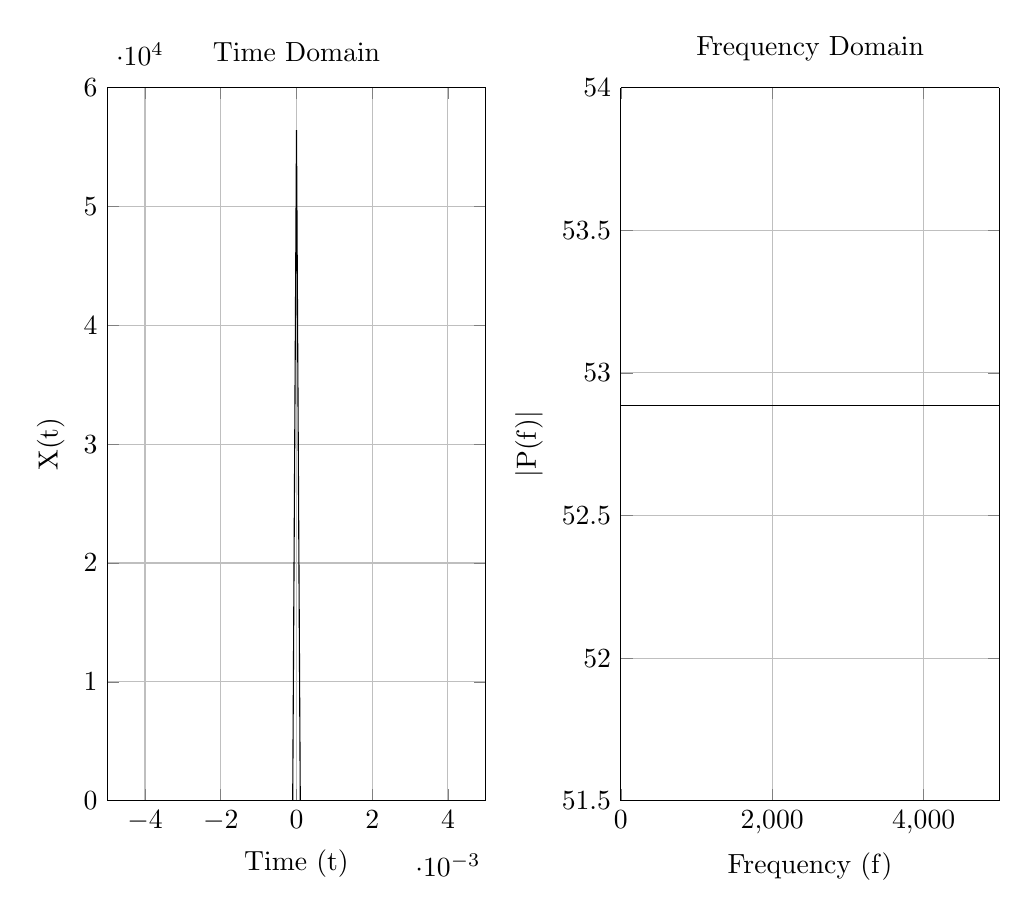
\begin{tikzpicture}

\begin{axis}[%
width=1.893in,
height=3.566in,
at={(0.818in,0.481in)},
scale only axis,
separate axis lines,
every outer x axis line/.append style={black},
every x tick label/.append style={font=\color{black}},
xmin=-0.005,
xmax=0.005,
xlabel={Time (t)},
xmajorgrids,
every outer y axis line/.append style={black},
every y tick label/.append style={font=\color{black}},
ymin=0,
ymax=60000,
ylabel={X(t)},
ymajorgrids,
axis background/.style={fill=white},
title={Time Domain}
]
\addplot [color=black,solid,forget plot]
  table[row sep=crcr]{%
-0.005	0\\
-0.0049	0\\
-0.0048	0\\
-0.0047	0\\
-0.0046	0\\
-0.0045	0\\
-0.0044	0\\
-0.0043	0\\
-0.0042	0\\
-0.0041	0\\
-0.004	0\\
-0.0039	0\\
-0.0038	0\\
-0.0037	0\\
-0.0036	0\\
-0.0035	0\\
-0.0034	0\\
-0.0033	0\\
-0.0032	0\\
-0.0031	0\\
-0.003	0\\
-0.0029	0\\
-0.0028	0\\
-0.0027	0\\
-0.0026	0\\
-0.0025	0\\
-0.0024	0\\
-0.0023	0\\
-0.0022	0\\
-0.0021	0\\
-0.002	0\\
-0.0019	0\\
-0.0018	0\\
-0.0017	0\\
-0.0016	0\\
-0.0015	0\\
-0.0014	0\\
-0.0013	0\\
-0.0012	0\\
-0.0011	0\\
-0.001	0\\
-0.0009	0\\
-0.0008	0\\
-0.0007	0\\
-0.0006	0\\
-0.0005	0\\
-0.0004	0\\
-0.0003	0\\
-0.0002	1.08051873719493e-169\\
-0.0001	2.09882811567613e-39\\
0	56418.9583547756\\
0.0001	2.09882811567613e-39\\
0.0002	1.08051873719493e-169\\
0.0003	0\\
0.0004	0\\
0.0005	0\\
0.0006	0\\
0.0007	0\\
0.0008	0\\
0.0009	0\\
0.001	0\\
0.0011	0\\
0.0012	0\\
0.0013	0\\
0.0014	0\\
0.0015	0\\
0.0016	0\\
0.0017	0\\
0.0018	0\\
0.0019	0\\
0.002	0\\
0.0021	0\\
0.0022	0\\
0.0023	0\\
0.0024	0\\
0.0025	0\\
0.0026	0\\
0.0027	0\\
0.0028	0\\
0.0029	0\\
0.003	0\\
0.0031	0\\
0.0032	0\\
0.0033	0\\
0.0034	0\\
0.0035	0\\
0.0036	0\\
0.0037	0\\
0.0038	0\\
0.0039	0\\
0.004	0\\
0.0041	0\\
0.0042	0\\
0.0043	0\\
0.0044	0\\
0.0045	0\\
0.0046	0\\
0.0047	0\\
0.0048	0\\
0.0049	0\\
0.005	0\\
};
\end{axis}

\begin{axis}[%
width=1.893in,
height=3.566in,
at={(3.386in,0.481in)},
scale only axis,
separate axis lines,
every outer x axis line/.append style={black},
every x tick label/.append style={font=\color{black}},
xmin=0,
xmax=5000,
xlabel={Frequency (f)},
xmajorgrids,
every outer y axis line/.append style={black},
every y tick label/.append style={font=\color{black}},
ymin=51.5,
ymax=54,
ylabel={$|$P(f)$|$},
ymajorgrids,
axis background/.style={fill=white},
title={Frequency Domain}
]
\addplot [color=black,solid,forget plot]
  table[row sep=crcr]{%
0	52.8843018801013\\
78.125	52.8843018801013\\
156.25	52.8843018801013\\
234.375	52.8843018801013\\
312.5	52.8843018801013\\
390.625	52.8843018801013\\
468.75	52.8843018801013\\
546.875	52.8843018801013\\
625	52.8843018801013\\
703.125	52.8843018801013\\
781.25	52.8843018801013\\
859.375	52.8843018801013\\
937.5	52.8843018801013\\
1015.625	52.8843018801013\\
1093.75	52.8843018801013\\
1171.875	52.8843018801013\\
1250	52.8843018801013\\
1328.125	52.8843018801013\\
1406.25	52.8843018801013\\
1484.375	52.8843018801013\\
1562.5	52.8843018801013\\
1640.625	52.8843018801013\\
1718.75	52.8843018801013\\
1796.875	52.8843018801013\\
1875	52.8843018801013\\
1953.125	52.8843018801013\\
2031.25	52.8843018801013\\
2109.375	52.8843018801013\\
2187.5	52.8843018801013\\
2265.625	52.8843018801013\\
2343.75	52.8843018801013\\
2421.875	52.8843018801013\\
2500	52.8843018801013\\
2578.125	52.8843018801013\\
2656.25	52.8843018801013\\
2734.375	52.8843018801013\\
2812.5	52.8843018801013\\
2890.625	52.8843018801013\\
2968.75	52.8843018801013\\
3046.875	52.8843018801013\\
3125	52.8843018801013\\
3203.125	52.8843018801013\\
3281.25	52.8843018801013\\
3359.375	52.8843018801013\\
3437.5	52.8843018801013\\
3515.625	52.8843018801013\\
3593.75	52.8843018801013\\
3671.875	52.8843018801013\\
3750	52.8843018801013\\
3828.125	52.8843018801013\\
3906.25	52.8843018801013\\
3984.375	52.8843018801013\\
4062.5	52.8843018801013\\
4140.625	52.8843018801013\\
4218.75	52.8843018801013\\
4296.875	52.8843018801013\\
4375	52.8843018801013\\
4453.125	52.8843018801013\\
4531.25	52.8843018801013\\
4609.375	52.8843018801013\\
4687.5	52.8843018801013\\
4765.625	52.8843018801013\\
4843.75	52.8843018801013\\
4921.875	52.8843018801013\\
5000	52.8843018801013\\
};
\end{axis}
\end{tikzpicture}%
% }
% \caption{An impulse }
% \label{fig:impulse1}
% \end{figure}

% \begin{figure}[H]
% \centering
% \tikzsetnextfilename{Impulse2}
% \scalebox{0.7}{
% % This file was created by matlab2tikz.
%
%The latest updates can be retrieved from
%  http://www.mathworks.com/matlabcentral/fileexchange/22022-matlab2tikz-matlab2tikz
%where you can also make suggestions and rate matlab2tikz.
%
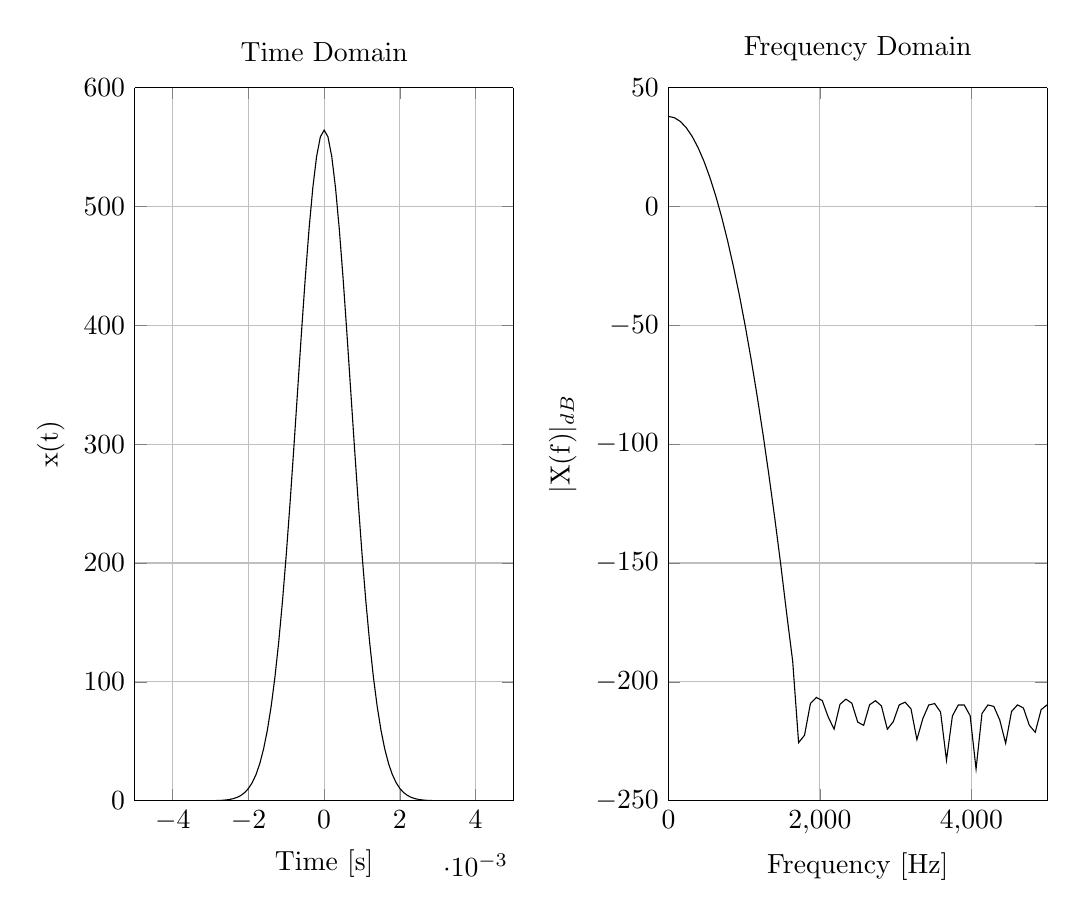
\begin{tikzpicture}

\begin{axis}[%
width=1.893in,
height=3.566in,
at={(0.818in,0.481in)},
scale only axis,
separate axis lines,
every outer x axis line/.append style={black},
every x tick label/.append style={font=\color{black}},
xmin=-0.005,
xmax=0.005,
xlabel={Time [s]},
xmajorgrids,
every outer y axis line/.append style={black},
every y tick label/.append style={font=\color{black}},
ymin=0,
ymax=600,
ylabel={x(t)},
ymajorgrids,
axis background/.style={fill=white},
title={Time Domain}
]
\addplot [color=black,solid,forget plot]
  table[row sep=crcr]{%
-0.005	7.83543326550864e-09\\
-0.0049	2.1086988109929e-08\\
-0.0048	5.56263034490542e-08\\
-0.0047	1.43833470140254e-07\\
-0.0046	3.64547250119098e-07\\
-0.0045	9.05652947954342e-07\\
-0.0044	2.2053823473417e-06\\
-0.0043	5.26405106104077e-06\\
-0.0042	1.23160204933418e-05\\
-0.0041	2.82445606028581e-05\\
-0.004	6.34911733593328e-05\\
-0.0039	0.00013989622447875\\
-0.0038	0.000302143144661123\\
-0.0037	0.000639637042267003\\
-0.0036	0.00132729842235829\\
-0.0035	0.00269971338869239\\
-0.0034	0.00538246051834033\\
-0.0033	0.0105186052217902\\
-0.0032	0.0201488177666178\\
-0.0031	0.0378316333982708\\
-0.003	0.0696265259733739\\
-0.0029	0.125605446260365\\
-0.0028	0.222103972102833\\
-0.0027	0.384962379927571\\
-0.0026	0.654025024861641\\
-0.0025	1.08914211517635\\
-0.0024	1.77782434043888\\
-0.0023	2.84450862126268\\
-0.0022	4.4610775324581\\
-0.0021	6.85782499990342\\
-0.002	10.333492677046\\
-0.0019	15.2623702177239\\
-0.0018	22.0958616660055\\
-0.0017	31.3555202484342\\
-0.0016	43.6145293169727\\
-0.0015	59.4651446118147\\
-0.0014	79.470853838639\\
-0.0013	104.103993398035\\
-0.0012	133.67217350177\\
-0.0011	168.239798896622\\
-0.001	207.553748710297\\
-0.0009	250.984287120181\\
-0.0008	297.492893128735\\
-0.0007	345.637430205269\\
-0.0006	393.621715857144\\
-0.0005	439.391289467723\\
-0.0004	480.770649419654\\
-0.0003	515.630454809482\\
-0.0002	542.067393552432\\
-0.0001	558.575803394468\\
0	564.189583547756\\
0.0001	558.575803394468\\
0.0002	542.067393552432\\
0.0003	515.630454809482\\
0.0004	480.770649419654\\
0.0005	439.391289467723\\
0.0006	393.621715857144\\
0.0007	345.637430205269\\
0.0008	297.492893128735\\
0.0009	250.984287120181\\
0.001	207.553748710297\\
0.0011	168.239798896622\\
0.0012	133.67217350177\\
0.0013	104.103993398035\\
0.0014	79.470853838639\\
0.0015	59.4651446118147\\
0.0016	43.6145293169727\\
0.0017	31.3555202484342\\
0.0018	22.0958616660055\\
0.0019	15.2623702177239\\
0.002	10.333492677046\\
0.0021	6.85782499990342\\
0.0022	4.4610775324581\\
0.0023	2.84450862126268\\
0.0024	1.77782434043888\\
0.0025	1.08914211517635\\
0.0026	0.654025024861641\\
0.0027	0.384962379927571\\
0.0028	0.222103972102833\\
0.0029	0.125605446260365\\
0.003	0.0696265259733739\\
0.0031	0.0378316333982708\\
0.0032	0.0201488177666178\\
0.0033	0.0105186052217902\\
0.0034	0.00538246051834033\\
0.0035	0.00269971338869239\\
0.0036	0.00132729842235829\\
0.0037	0.000639637042267003\\
0.0038	0.000302143144661123\\
0.0039	0.00013989622447875\\
0.004	6.34911733593328e-05\\
0.0041	2.82445606028581e-05\\
0.0042	1.23160204933418e-05\\
0.0043	5.26405106104077e-06\\
0.0044	2.2053823473417e-06\\
0.0045	9.05652947954342e-07\\
0.0046	3.64547250119098e-07\\
0.0047	1.43833470140254e-07\\
0.0048	5.56263034490542e-08\\
0.0049	2.1086988109929e-08\\
0.005	7.83543326550864e-09\\
};
\end{axis}

\begin{axis}[%
width=1.893in,
height=3.566in,
at={(3.486in,0.481in)},
scale only axis,
separate axis lines,
every outer x axis line/.append style={black},
every x tick label/.append style={font=\color{black}},
xmin=0,
xmax=5000,
xlabel={Frequency [Hz]},
xmajorgrids,
every outer y axis line/.append style={black},
every y tick label/.append style={font=\color{black}},
ymin=-250,
ymax=50,
ylabel={$|$X(f)$|_{dB}$},
ymajorgrids,
axis background/.style={fill=white},
title={Frequency Domain}
]
\addplot [color=black,solid,forget plot]
  table[row sep=crcr]{%
0	37.855800607035\\
78.125	37.3325688284896\\
156.25	35.7628734928005\\
234.375	33.1467146000018\\
312.5	29.4840921501025\\
390.625	24.7750061430162\\
468.75	19.0194565789488\\
546.875	12.2174434575596\\
625	4.36896677915439\\
703.125	-4.52597345561197\\
781.25	-14.4673772518028\\
859.375	-25.4552445897236\\
937.5	-37.4895755234318\\
1015.625	-50.5703699969464\\
1093.75	-64.6976273724835\\
1171.875	-79.8713544451494\\
1250	-96.0915066331747\\
1328.125	-113.358286926916\\
1406.25	-131.671567607568\\
1484.375	-151.019248978027\\
1562.5	-171.606034051156\\
1640.625	-191.298724926027\\
1718.75	-225.533783109023\\
1796.875	-222.456448217508\\
1875	-209.062180332166\\
1953.125	-206.532411589981\\
2031.25	-207.856157758439\\
2109.375	-214.736384202754\\
2187.5	-219.848325923748\\
2265.625	-209.428742938503\\
2343.75	-207.254882215146\\
2421.875	-208.951932664328\\
2500	-216.95411287222\\
2578.125	-218.25310330109\\
2656.25	-209.617667296797\\
2734.375	-207.91133374244\\
2812.5	-210.107422986409\\
2890.625	-219.905291162533\\
2968.75	-216.759195752299\\
3046.875	-209.700318071509\\
3125	-208.524028611558\\
3203.125	-211.338813793137\\
3281.25	-224.263264601684\\
3359.375	-215.446664808203\\
3437.5	-209.718709732226\\
3515.625	-209.118734186728\\
3593.75	-212.682258138089\\
3671.875	-232.924718510278\\
3750	-214.310438871519\\
3828.125	-209.709871268567\\
3906.25	-209.709910487451\\
3984.375	-214.208027867961\\
4062.5	-236.634945273642\\
4140.625	-213.312537485231\\
4218.75	-209.697651144571\\
4296.875	-210.317761964784\\
4375	-215.999627109929\\
4453.125	-225.809711386653\\
4531.25	-212.440350012178\\
4609.375	-209.684317861375\\
4687.5	-210.964704832857\\
4765.625	-218.217317888788\\
4843.75	-221.201021704194\\
4921.875	-211.664214485549\\
5000	-209.679117352519\\
};
\end{axis}
\end{tikzpicture}%}
% \caption{An impulse}
% \label{fig:impulse2}
% \end{figure}

If the coil hits the back plate it will create an impulse which will give an energy spike in a wider frequency range dependent on the impulse and the speaker itself as seen on \autoref{fig:impulse}. The shorter the impulse, the wider the frequency range as compared in the differences seen between \autoref{fig:impulse1} and \autoref{fig:impulse2}.  

\begin{figure}[H]
\begin{subfigure}[t]{0.47\textwidth}
\centering
\tikzsetnextfilename{Impulse1}
\scalebox{0.6}{
% This file was created by matlab2tikz.
%
%The latest updates can be retrieved from
%  http://www.mathworks.com/matlabcentral/fileexchange/22022-matlab2tikz-matlab2tikz
%where you can also make suggestions and rate matlab2tikz.
%
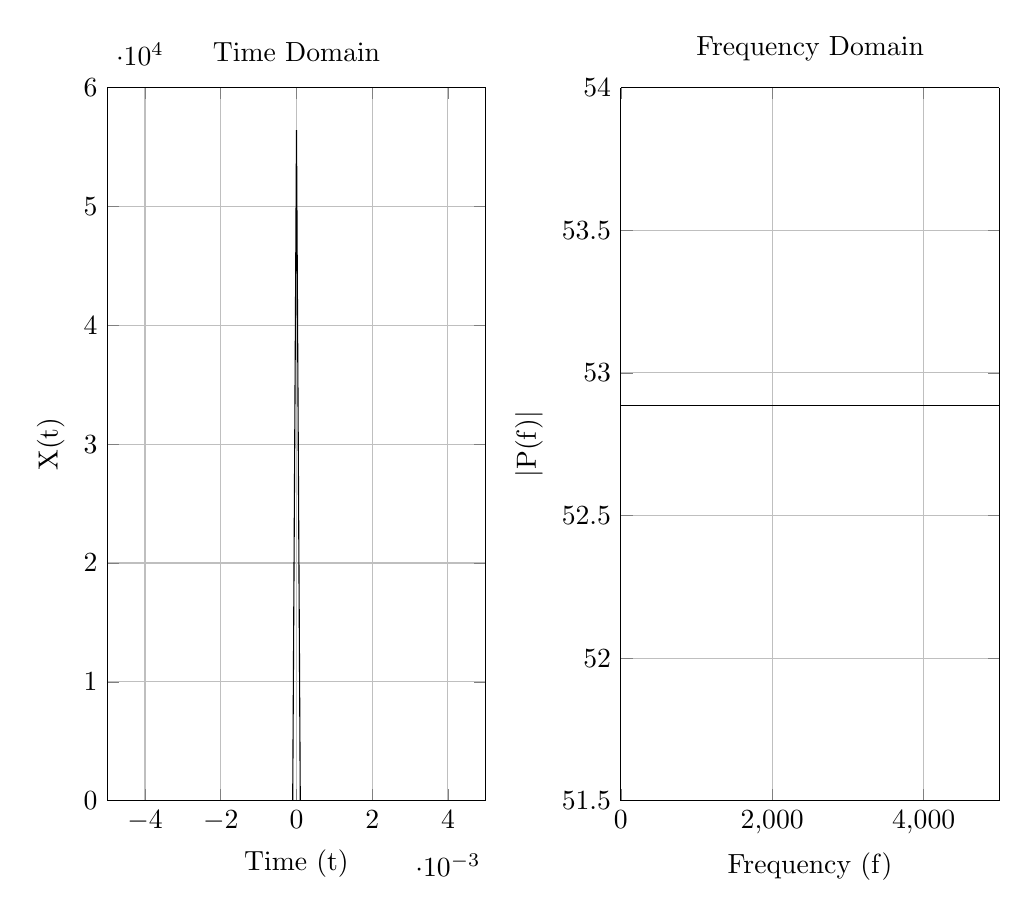
\begin{tikzpicture}

\begin{axis}[%
width=1.893in,
height=3.566in,
at={(0.818in,0.481in)},
scale only axis,
separate axis lines,
every outer x axis line/.append style={black},
every x tick label/.append style={font=\color{black}},
xmin=-0.005,
xmax=0.005,
xlabel={Time (t)},
xmajorgrids,
every outer y axis line/.append style={black},
every y tick label/.append style={font=\color{black}},
ymin=0,
ymax=60000,
ylabel={X(t)},
ymajorgrids,
axis background/.style={fill=white},
title={Time Domain}
]
\addplot [color=black,solid,forget plot]
  table[row sep=crcr]{%
-0.005	0\\
-0.0049	0\\
-0.0048	0\\
-0.0047	0\\
-0.0046	0\\
-0.0045	0\\
-0.0044	0\\
-0.0043	0\\
-0.0042	0\\
-0.0041	0\\
-0.004	0\\
-0.0039	0\\
-0.0038	0\\
-0.0037	0\\
-0.0036	0\\
-0.0035	0\\
-0.0034	0\\
-0.0033	0\\
-0.0032	0\\
-0.0031	0\\
-0.003	0\\
-0.0029	0\\
-0.0028	0\\
-0.0027	0\\
-0.0026	0\\
-0.0025	0\\
-0.0024	0\\
-0.0023	0\\
-0.0022	0\\
-0.0021	0\\
-0.002	0\\
-0.0019	0\\
-0.0018	0\\
-0.0017	0\\
-0.0016	0\\
-0.0015	0\\
-0.0014	0\\
-0.0013	0\\
-0.0012	0\\
-0.0011	0\\
-0.001	0\\
-0.0009	0\\
-0.0008	0\\
-0.0007	0\\
-0.0006	0\\
-0.0005	0\\
-0.0004	0\\
-0.0003	0\\
-0.0002	1.08051873719493e-169\\
-0.0001	2.09882811567613e-39\\
0	56418.9583547756\\
0.0001	2.09882811567613e-39\\
0.0002	1.08051873719493e-169\\
0.0003	0\\
0.0004	0\\
0.0005	0\\
0.0006	0\\
0.0007	0\\
0.0008	0\\
0.0009	0\\
0.001	0\\
0.0011	0\\
0.0012	0\\
0.0013	0\\
0.0014	0\\
0.0015	0\\
0.0016	0\\
0.0017	0\\
0.0018	0\\
0.0019	0\\
0.002	0\\
0.0021	0\\
0.0022	0\\
0.0023	0\\
0.0024	0\\
0.0025	0\\
0.0026	0\\
0.0027	0\\
0.0028	0\\
0.0029	0\\
0.003	0\\
0.0031	0\\
0.0032	0\\
0.0033	0\\
0.0034	0\\
0.0035	0\\
0.0036	0\\
0.0037	0\\
0.0038	0\\
0.0039	0\\
0.004	0\\
0.0041	0\\
0.0042	0\\
0.0043	0\\
0.0044	0\\
0.0045	0\\
0.0046	0\\
0.0047	0\\
0.0048	0\\
0.0049	0\\
0.005	0\\
};
\end{axis}

\begin{axis}[%
width=1.893in,
height=3.566in,
at={(3.386in,0.481in)},
scale only axis,
separate axis lines,
every outer x axis line/.append style={black},
every x tick label/.append style={font=\color{black}},
xmin=0,
xmax=5000,
xlabel={Frequency (f)},
xmajorgrids,
every outer y axis line/.append style={black},
every y tick label/.append style={font=\color{black}},
ymin=51.5,
ymax=54,
ylabel={$|$P(f)$|$},
ymajorgrids,
axis background/.style={fill=white},
title={Frequency Domain}
]
\addplot [color=black,solid,forget plot]
  table[row sep=crcr]{%
0	52.8843018801013\\
78.125	52.8843018801013\\
156.25	52.8843018801013\\
234.375	52.8843018801013\\
312.5	52.8843018801013\\
390.625	52.8843018801013\\
468.75	52.8843018801013\\
546.875	52.8843018801013\\
625	52.8843018801013\\
703.125	52.8843018801013\\
781.25	52.8843018801013\\
859.375	52.8843018801013\\
937.5	52.8843018801013\\
1015.625	52.8843018801013\\
1093.75	52.8843018801013\\
1171.875	52.8843018801013\\
1250	52.8843018801013\\
1328.125	52.8843018801013\\
1406.25	52.8843018801013\\
1484.375	52.8843018801013\\
1562.5	52.8843018801013\\
1640.625	52.8843018801013\\
1718.75	52.8843018801013\\
1796.875	52.8843018801013\\
1875	52.8843018801013\\
1953.125	52.8843018801013\\
2031.25	52.8843018801013\\
2109.375	52.8843018801013\\
2187.5	52.8843018801013\\
2265.625	52.8843018801013\\
2343.75	52.8843018801013\\
2421.875	52.8843018801013\\
2500	52.8843018801013\\
2578.125	52.8843018801013\\
2656.25	52.8843018801013\\
2734.375	52.8843018801013\\
2812.5	52.8843018801013\\
2890.625	52.8843018801013\\
2968.75	52.8843018801013\\
3046.875	52.8843018801013\\
3125	52.8843018801013\\
3203.125	52.8843018801013\\
3281.25	52.8843018801013\\
3359.375	52.8843018801013\\
3437.5	52.8843018801013\\
3515.625	52.8843018801013\\
3593.75	52.8843018801013\\
3671.875	52.8843018801013\\
3750	52.8843018801013\\
3828.125	52.8843018801013\\
3906.25	52.8843018801013\\
3984.375	52.8843018801013\\
4062.5	52.8843018801013\\
4140.625	52.8843018801013\\
4218.75	52.8843018801013\\
4296.875	52.8843018801013\\
4375	52.8843018801013\\
4453.125	52.8843018801013\\
4531.25	52.8843018801013\\
4609.375	52.8843018801013\\
4687.5	52.8843018801013\\
4765.625	52.8843018801013\\
4843.75	52.8843018801013\\
4921.875	52.8843018801013\\
5000	52.8843018801013\\
};
\end{axis}
\end{tikzpicture}%}
\caption{Impulse 1}
\label{fig:impulse1}
\end{subfigure}
\hspace{6mm} 
\begin{subfigure}[t]{0.47\textwidth}
\centering
\tikzsetnextfilename{Impulse2}
\scalebox{0.6}{
% This file was created by matlab2tikz.
%
%The latest updates can be retrieved from
%  http://www.mathworks.com/matlabcentral/fileexchange/22022-matlab2tikz-matlab2tikz
%where you can also make suggestions and rate matlab2tikz.
%
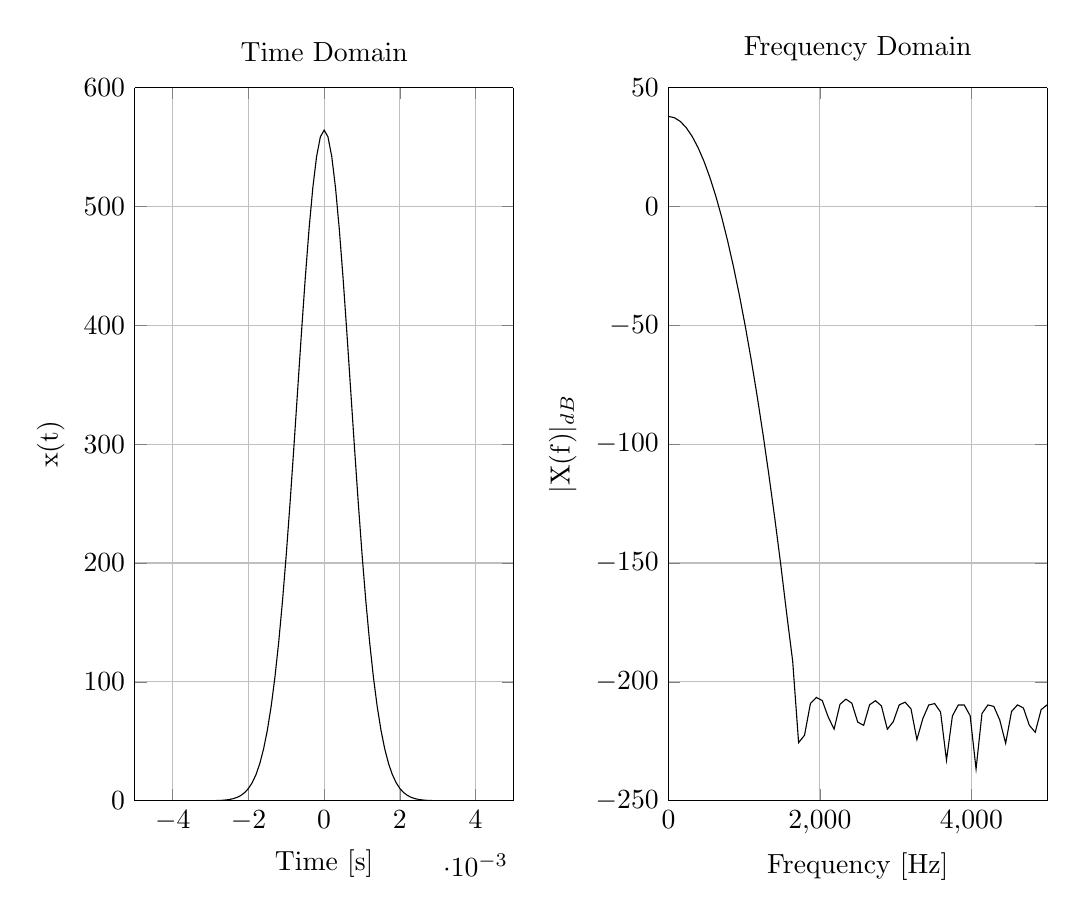
\begin{tikzpicture}

\begin{axis}[%
width=1.893in,
height=3.566in,
at={(0.818in,0.481in)},
scale only axis,
separate axis lines,
every outer x axis line/.append style={black},
every x tick label/.append style={font=\color{black}},
xmin=-0.005,
xmax=0.005,
xlabel={Time [s]},
xmajorgrids,
every outer y axis line/.append style={black},
every y tick label/.append style={font=\color{black}},
ymin=0,
ymax=600,
ylabel={x(t)},
ymajorgrids,
axis background/.style={fill=white},
title={Time Domain}
]
\addplot [color=black,solid,forget plot]
  table[row sep=crcr]{%
-0.005	7.83543326550864e-09\\
-0.0049	2.1086988109929e-08\\
-0.0048	5.56263034490542e-08\\
-0.0047	1.43833470140254e-07\\
-0.0046	3.64547250119098e-07\\
-0.0045	9.05652947954342e-07\\
-0.0044	2.2053823473417e-06\\
-0.0043	5.26405106104077e-06\\
-0.0042	1.23160204933418e-05\\
-0.0041	2.82445606028581e-05\\
-0.004	6.34911733593328e-05\\
-0.0039	0.00013989622447875\\
-0.0038	0.000302143144661123\\
-0.0037	0.000639637042267003\\
-0.0036	0.00132729842235829\\
-0.0035	0.00269971338869239\\
-0.0034	0.00538246051834033\\
-0.0033	0.0105186052217902\\
-0.0032	0.0201488177666178\\
-0.0031	0.0378316333982708\\
-0.003	0.0696265259733739\\
-0.0029	0.125605446260365\\
-0.0028	0.222103972102833\\
-0.0027	0.384962379927571\\
-0.0026	0.654025024861641\\
-0.0025	1.08914211517635\\
-0.0024	1.77782434043888\\
-0.0023	2.84450862126268\\
-0.0022	4.4610775324581\\
-0.0021	6.85782499990342\\
-0.002	10.333492677046\\
-0.0019	15.2623702177239\\
-0.0018	22.0958616660055\\
-0.0017	31.3555202484342\\
-0.0016	43.6145293169727\\
-0.0015	59.4651446118147\\
-0.0014	79.470853838639\\
-0.0013	104.103993398035\\
-0.0012	133.67217350177\\
-0.0011	168.239798896622\\
-0.001	207.553748710297\\
-0.0009	250.984287120181\\
-0.0008	297.492893128735\\
-0.0007	345.637430205269\\
-0.0006	393.621715857144\\
-0.0005	439.391289467723\\
-0.0004	480.770649419654\\
-0.0003	515.630454809482\\
-0.0002	542.067393552432\\
-0.0001	558.575803394468\\
0	564.189583547756\\
0.0001	558.575803394468\\
0.0002	542.067393552432\\
0.0003	515.630454809482\\
0.0004	480.770649419654\\
0.0005	439.391289467723\\
0.0006	393.621715857144\\
0.0007	345.637430205269\\
0.0008	297.492893128735\\
0.0009	250.984287120181\\
0.001	207.553748710297\\
0.0011	168.239798896622\\
0.0012	133.67217350177\\
0.0013	104.103993398035\\
0.0014	79.470853838639\\
0.0015	59.4651446118147\\
0.0016	43.6145293169727\\
0.0017	31.3555202484342\\
0.0018	22.0958616660055\\
0.0019	15.2623702177239\\
0.002	10.333492677046\\
0.0021	6.85782499990342\\
0.0022	4.4610775324581\\
0.0023	2.84450862126268\\
0.0024	1.77782434043888\\
0.0025	1.08914211517635\\
0.0026	0.654025024861641\\
0.0027	0.384962379927571\\
0.0028	0.222103972102833\\
0.0029	0.125605446260365\\
0.003	0.0696265259733739\\
0.0031	0.0378316333982708\\
0.0032	0.0201488177666178\\
0.0033	0.0105186052217902\\
0.0034	0.00538246051834033\\
0.0035	0.00269971338869239\\
0.0036	0.00132729842235829\\
0.0037	0.000639637042267003\\
0.0038	0.000302143144661123\\
0.0039	0.00013989622447875\\
0.004	6.34911733593328e-05\\
0.0041	2.82445606028581e-05\\
0.0042	1.23160204933418e-05\\
0.0043	5.26405106104077e-06\\
0.0044	2.2053823473417e-06\\
0.0045	9.05652947954342e-07\\
0.0046	3.64547250119098e-07\\
0.0047	1.43833470140254e-07\\
0.0048	5.56263034490542e-08\\
0.0049	2.1086988109929e-08\\
0.005	7.83543326550864e-09\\
};
\end{axis}

\begin{axis}[%
width=1.893in,
height=3.566in,
at={(3.486in,0.481in)},
scale only axis,
separate axis lines,
every outer x axis line/.append style={black},
every x tick label/.append style={font=\color{black}},
xmin=0,
xmax=5000,
xlabel={Frequency [Hz]},
xmajorgrids,
every outer y axis line/.append style={black},
every y tick label/.append style={font=\color{black}},
ymin=-250,
ymax=50,
ylabel={$|$X(f)$|_{dB}$},
ymajorgrids,
axis background/.style={fill=white},
title={Frequency Domain}
]
\addplot [color=black,solid,forget plot]
  table[row sep=crcr]{%
0	37.855800607035\\
78.125	37.3325688284896\\
156.25	35.7628734928005\\
234.375	33.1467146000018\\
312.5	29.4840921501025\\
390.625	24.7750061430162\\
468.75	19.0194565789488\\
546.875	12.2174434575596\\
625	4.36896677915439\\
703.125	-4.52597345561197\\
781.25	-14.4673772518028\\
859.375	-25.4552445897236\\
937.5	-37.4895755234318\\
1015.625	-50.5703699969464\\
1093.75	-64.6976273724835\\
1171.875	-79.8713544451494\\
1250	-96.0915066331747\\
1328.125	-113.358286926916\\
1406.25	-131.671567607568\\
1484.375	-151.019248978027\\
1562.5	-171.606034051156\\
1640.625	-191.298724926027\\
1718.75	-225.533783109023\\
1796.875	-222.456448217508\\
1875	-209.062180332166\\
1953.125	-206.532411589981\\
2031.25	-207.856157758439\\
2109.375	-214.736384202754\\
2187.5	-219.848325923748\\
2265.625	-209.428742938503\\
2343.75	-207.254882215146\\
2421.875	-208.951932664328\\
2500	-216.95411287222\\
2578.125	-218.25310330109\\
2656.25	-209.617667296797\\
2734.375	-207.91133374244\\
2812.5	-210.107422986409\\
2890.625	-219.905291162533\\
2968.75	-216.759195752299\\
3046.875	-209.700318071509\\
3125	-208.524028611558\\
3203.125	-211.338813793137\\
3281.25	-224.263264601684\\
3359.375	-215.446664808203\\
3437.5	-209.718709732226\\
3515.625	-209.118734186728\\
3593.75	-212.682258138089\\
3671.875	-232.924718510278\\
3750	-214.310438871519\\
3828.125	-209.709871268567\\
3906.25	-209.709910487451\\
3984.375	-214.208027867961\\
4062.5	-236.634945273642\\
4140.625	-213.312537485231\\
4218.75	-209.697651144571\\
4296.875	-210.317761964784\\
4375	-215.999627109929\\
4453.125	-225.809711386653\\
4531.25	-212.440350012178\\
4609.375	-209.684317861375\\
4687.5	-210.964704832857\\
4765.625	-218.217317888788\\
4843.75	-221.201021704194\\
4921.875	-211.664214485549\\
5000	-209.679117352519\\
};
\end{axis}
\end{tikzpicture}%}
\caption{Impulse 2}
\label{fig:impulse2}
\end{subfigure}
\caption{Two different impulses and there frequency response.}
\label{fig:impulse}
\end{figure}
Besides the characteristics of the impulse the loudspeaker will act as a low-pass filter so the frequency response of an impulse will always resemble the frequency response of \autoref{fig:impulse2} of some sort. However when playing music these impulses will be difficult to estimate through a spectrum analysis, because music in itself can consist of impulses.     


%that occurs at playback. The vibrations occurs because the  If the vibration. the sound radiated from the loudspeaker enclosure